\documentclass[12pt,a4paper,oneside]{book} %%%%%%%%%%%%%%%%%%%%%%%%%%%%%%%%%%%%%%%%%%%%%%%%%

%%% preample %%%%%%%%%%%%%%%%%%%%%%%%%%%%%%%%%%%%%%%%%%%%%%%%%%%%%%%%%%%%%%%%%%


%%% packages %%%%%%%%%%%%%%%%%%%%%%%%%%%%%%%%%%%%%%%%%%%%%%%%%%%%%%%%%%%%%%%%%%

\usepackage[T1]{fontenc}        % euro quality fonts [T1] (togeth. w/ textcomp)
\usepackage{textcomp, amssymb}  % additional symbols (there are more packages)
\usepackage[utf8]{inputenc}   % umlaute in input file
\usepackage[english]{babel}     % newgerman: Worttrennung, Befehle f�r Umlaute
\usepackage{anysize}            % margin package sets tighter margins

\usepackage[a4paper,top=2cm,bottom=2cm,left=2cm,right=2cm]{geometry}

\usepackage{ifpdf}              % if pdflatex then ... else ...
%newer versions of latex don't need pdftex and dvips argument respectively
\ifpdf
  \usepackage{aeguill}          % PS converted CM fonts for better acro preview
  \usepackage[pdftex]{graphicx} % graphics packages
  \usepackage[pdftex]{color}    % color packages
  \usepackage[pdftex]{hyperref}
\else
  \usepackage[dvips]{graphicx}  % graphics packages
  \usepackage[dvips]{hyperref}
\fi

%%% style and finetuning %%%%%%%%%%%%%%%%%%%%%%%%%%%%%%%%%%%%%%%%%%%%%%%%%%%%%%

% pagestyle
\pagestyle{plain}               % headings, empty, plain

\hypersetup{colorlinks=false}   % don't print colored links on paper

% no indentation for paragraphs and space inbetween paragraphs  (euro standard)
\setlength{\parindent}{0pt}
\setlength{\parskip}{5pt plus 2pt minus 1pt}

\renewcommand{\baselinestretch}{1.05}

\graphicspath{ {./images/} }

%%% hacks %%%%%%%%%%%%%%%%%%%%%%%%%%%%%%%%%%%%%%%%%%%%%%%%%%%%%%%%%%%%%%%%%%%%%

% hyperref must be (almost) last command of preample
% E.g. The \href{http://www.ctan.org}{CTAN} website.
% E.g. \author{First- Lastname $<$\href{mailto: email@domain}{email@domain}$>$}

\ifpdf
  \usepackage[pdftex]{hyperref}
\else
  \usepackage[dvips]{hyperref}
\fi
\hypersetup{colorlinks=false}   % don't print colors on paper
\usepackage{float}

\newcommand{\chapterimage}{nothing}

\newcommand{\newchapter}[2]{
    \renewcommand{\chapterimage}{#2}
    \chapter{#1}
}

\makeatletter
\renewcommand*{\@makechapterhead}[1]{
  \begin{figure}[H]
  \centering
  \thispagestyle{empty}
  \includegraphics[width=\textwidth,height=\textheight,keepaspectratio]{\chapterimage}
  \end{figure}
  \newpage
  {\Huge Chapter \thechapter: #1}
}
\makeatother


\begin{document}
%%% tile page %%%%%%%%%%%%%%%%%%%%%%%%%%%%%%%%%%%%%%%%%%%%%%%%%%%%%%%%%%%%%%%%%

\begin{titlepage}
\thispagestyle{empty}

\hrule
\begin{center}
{\bf\LARGE Hero History Apocrypha}

%\vspace{2cm}
%\begin{figure}[!htbp]
% \centering
% 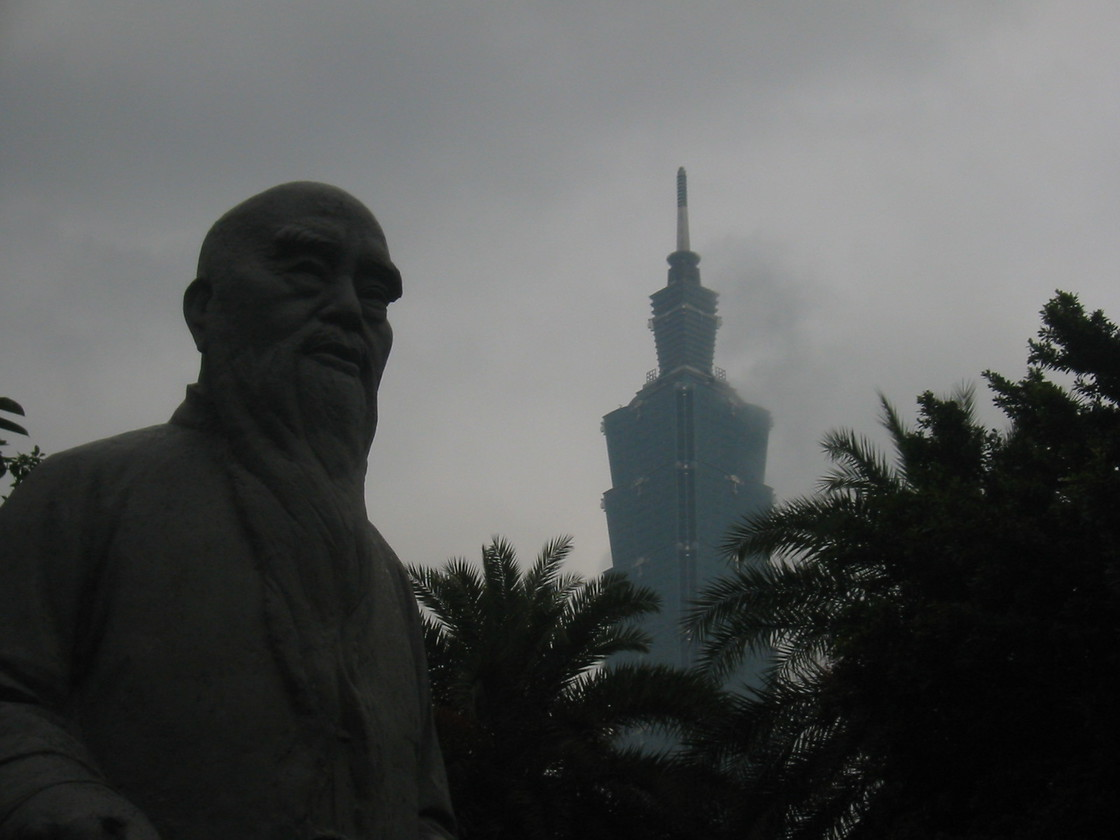
\includegraphics[width=1.0\textwidth]{images/cover_medium}
%\end{figure}

\end{center}
\end{titlepage}


\newpage %%%%%%%%%%%%%%%%%%%%%%%%%%%%%%%%%%%%%%%%%%%%%%%%%%%%%%%%%%%%%%%%%%%%%%

\setcounter{page}{1}\pagenumbering{roman}

\tableofcontents

\newpage

\setcounter{page}{1}\pagenumbering{arabic}

\part{Uesato Hinata is a Miko}
        
\newchapter{The Mikos}{uhimi-ch1-cover.jpg}

No human truly believes they will will one day die.

According to a literature-loving friend of mine, even Sigmund Freud, the founder of psychoanalysis, has said: ``As humans are incapable of accurately imagining their own death, they are thus incapable of truly believing their own death.''

Life is akin to walking on thin ice. Nobody knows when that ``death'' people don't even believe in will open its sinister jaws and swallow them.

Even the disaster that occurred in 2015 --- not that it was something as simple as disaster; I simply can't find a better expression --- was not something that anyone would believe would happen. But it did.

Vertexes. That was the name of the monsters that descended from the heavens, taking the lives of many people and destroying civilisation.

Amidst all that, special powers sprouted in some girls.

The power to stand against the Vertexes. The girls who manifested that power were called Heroes.

The power to receive oracles in order to guide the Heroes and the populace. The girls who manifested that power were called Mikos.

I, Aki Masuzu, was one of the Mikos.

``Cold! No way! I can't handle any more! I'm gonna die!''

2019, March. The winter cold still lingered strongly in those early spring days. I screamed those words out during our Mikos' daily waterfall purification ritual and dashed out of the waterfall.

``Aki-san, it hasn't even been two minutes yet...''  Those words, accompanied by a wry smile, came from Uesato Hinata, who was also purifying herself under the waterfall. That girl was also a Miko, and a year younger than me.

``Two minutes is enough time for instant noodles to cook! Besides, I've got a slender body with little body fat, so I'm weak against the cold. And we've got someone unforgivable here!''  I immediately started running towards that unforgivable ``someone''.

``Eh, Aki-san!? Where are you going?''  Uesato-chan followed right behind me.

I threw open the door to the Taisha public bath.

Behind that door someone was leisurely soaking in the bath while we Mikos were suffering under the cold waterfall.

``I'm going to take a bath too!'' I said as I jump into the bath.

``Wait, Aki-senpai! Please don't come in all of a sudden!''  With her face and hair wet from the splashing water, the girl - Hanamoto Yoshika - was glaring at me. I silently ignored her glare.

``Hee-hee, would it be okay if I joined as well? Purification by water really chills the body.''  Uesato-chan appeared from behind and came in as well.

``Mhm, it's fine. You come in too, Uesato-chan.''

``Why are you giving her permission, Aki-senpai? Please get out already, you're making the bath cramped.'' Hanamoto-chan glared at me.

``Ah, sorry. I'll leave if I'm bothering you,'' said Uesato-chan.

``No, it's fine. Uesato-san, soak into the bath and warm up. It would be bad if you caught a cold.''

``Wait a minute, Hanamoto-chan. Aren't you treating me and Uesato-chan way too differently?''

``Senpai, different people absolutely do not have the same worth. Doubly so for subjective worth in someone's eyes.''

``I have a feeling I'm being ridiculed by big words!''  I scooped up some water from the bath and splashed it at Yoshika. But that didn't manage to distort her cold expression even a little. Though since she didn't seriously try to chase me out of the bath, I didn't think Yoshika-chan actually hated me.

...Probably.

...Definitely.

...I hope so.

``Besides, it's your fault for being allowed not to stand under the waterfalls and getting to soak in the bath, Hanamoto-chan.''

Hanamoto-chan was a Miko, just like me and Uesato-chan, so she would also need to purify her body daily to serve the gods. She met my displeased look with a calm answer.  ``I can't enter water.''

That's right. She had aquaphobia. Even entering a warm knee-deep bath was a recent achievement for her; she couldn't possibly stand under a waterfall.

A while ago, when she first came under a waterfall, Hanamoto-chan threw up and lost consciousness. After that, she was allowed to purify herself in just bathwater.

``Warm bathwater is plenty enough for purifying the body. We're not monks in training, there's no need for asceticism. And besides, rituals get simplified all the time. When you enter a shrine, all you do is rinse your hands and mouth, right? That's a simplified purification ritual too, can't we do just that?''

``Oh... That's the kind of knowledge I'd expect from someone who's family owns a shrine. How about you let the higher-ups hear that reasoning of yours?''

Hanamoto-chan was born and raised at a shrine. Because of that, she knew a lot about religious stuff like gods and rituals.

``It's pointless. The things they and I believe in are different. They have their own beliefs,'' she said in a cold tone, shaking her head.

Uesato-chan folded her arms, listening to our talking. Stop it, your breasts are already too big for a middle-schooler and you're emphasizing them even more.  ``You're right... I'll talk to the Taisha priests. Doing waterfall purification in the cold months isn't good for the Mikos' wellbeing. I'll ask them to allow everyone to use bathing for purification just like Hanamoto-san.''

``Oh, that's good! The adults ought to listen if it's coming from you, Uesato-chan!''

When all was said and done, Uesato-chan had the strongest powers of all the Mikos. She was the most important Miko to the Taisha. They were bound to answer a request from her.

``If they insist that waterfall purification is necessary, I'll do it by myself. As long as that gets the other Mikos excused from it....''

``Eh? Uesato-chan, are you saying you're going to stand under the waterfalls all on your own?''

``Yes. If it's necessary.''

I let out a powerful sigh.  ``Then I'll do it with you too. I can't let a girl younger than me do something so harsh by herself.''

Uesato-chan calmly smiled and bowed her head.

Ah, jeez. I had wanted to get away from those waterfalls, but wasn't able to do it in the end. Her words would probably go through, too. Uesato-chan had managed to find a way for both me and the adults to save face and had found a compromise neither of us could refuse.

When Uesato-chan talked, this kind of stuff happened sometimes. She was on our side, but also on the Taisha's, so she tried to settle things as neutrally and conflict-free as possible.

Even if she had to pay the price before anybody else. It was really brave of Uesato-chan to be able to do that, but at the same time somewhat scary.

Now, three and a half years after 2015 when the Vertexes appeared and destroyed most of Japan, humans still survived in just a few places, or so we were told. The reason for that uncertain ``we were told'' is that we currently lived in Shikoku, but could not see the state of things outside it.

Shinju, said to be a congregation of the earthly gods, and a barrier that protects against Vertex attacks, had appeared in Shikoku. Thanks to them, humans could still live in this land. But because it was swarming with Vertexes outside the barrier, going outside it --- and thus, outside Shikoku --- was impossible. Which was why we didn't know how things are outside.

Right now, the organisation formed by the priesthood known as the Taisha [Grand Shrine] was in charge of the Vertex countermeasures.

The Taisha had gathered Heroes and Mikos under their control to stand against the Vertexes. The five Heroes in Shikoku all lived in their base, Marugame castle in the Kagawa prefecture. There were more Mikos than Heroes, and aside from Uesato-chan, who lived in the Marugame castle to keep watch over the Heroes, they all lived in Taisha facilities.

Among the Mikos, there were three central figures.

The first was Uesato Hinata. The best friend of Nogi Wakaba, a Hero, she guided her during the initial Vertex appearance. She had the strongest power of all the Mikos. She was in her second year of middle school and a year younger than me, but her breasts were big. They were huge.

The other one was Hanamoto Yoshika. She found Koori Chikage, a Hero, and she came from a shrine in the first place. She was a second-year, just like Uesato-chan. By the way, the kanji in her name read Yoshika, not Mika.

And then there was me, Aki Masuzu. I was a vivacious third-year who found the Heroes Doi Tamako and Iyojima Anzu! I was older than Uesato-chan and Hanamoto-chan, so I tried to act like their big sister, but I couldn't shake off the feeling Hanamoto-chan treats me really rudely. I knew I had to show her that I'm the older one here, but unfortunately I hadn't quite had the chance yet. Plus, since Uesato-chan was more proficient as a Miko and Hanamoto-chan was more knowledgeable, who knew if I'd ever get that chance.

By the way, aside from the four Heroes I already mentioned, there was another one. Takashima Yuuna was guided by a Miko called Karasuma Kumiko, but she was a lot older than the rest of us and it seemed she'd already lost her Miko powers. Right now, she served as a priestess at the Taisha.

Uesato-chan usually lived in the Marugame castle, but right now she was visiting the Taisha for a change.

``By the way, Uesato-chan, why are you at the Taisha today?'' I asked her after the bath while drying my hair.

``The Heroes will be going to explore what's outside of the barrier soon, so I was called in for a meeting to confirm the route.''

``...So they really are going to explore what's outside, huh.''

A little ago, the Heroes had fought and won a massive battle with the Vertexes, the Battle of the Marugame castle. For a while after that, the Vertex attacks on Shikoku stopped. So a plan to send the Heroes to scout outside of the barrier in this brief moment of peace for Shikoku was proposed. And it seemed they were going through with it.

Three and a half years had passed since the barrier protecting Shikoku formed. In that time, no exploration outside of Shikoku could be made because of the Vertex threat.

Until last summer, it was known that there were still people alive in Suwa in the Nagano prefecture, but it'd been half a year since that and nobody knew what was going on with Suwa now.

Hanamoto-chan, while changing, frowned anxiously.  ``Uesato-san, is it really okay for people to go outside the barrier? There's a rumour that outside of the barrier is brimming with toxins...''

``Yesterday, the Heroes went just slightly beyond the barrier to check the state of the earth, atmosphere and water. And not only is it not contaminated, the ecological situation is even better than before.''

Uesato-chan's words didn't make Hanamoto-chan's expression any brighter. It seemed her worries hadn't been dispelled.

With our morning purification ritual done, me and Hanamoto-chan go to the classroom. Uesato-chan goes to talk with the adults about the Heroes' expedition.

By the time we reached the classroom, most of the other Mikos were already there. It looked like we ended up late because we went to the bath after the waterfalls.

When it was time to start the lesson, a woman in her twenties wearing a white robe entered the classroom. It was Karasuma Kumiko, the former Miko. Aside from her work as a priestess, Karasuma-sensei was also the Mikos' teacher.

``Uh, alright, let's begin the lesson.''  Karasuma-sensei was almost listless. Apparently, she had been a graduate student before she entered the Taisha as a Miko, and quite a brilliant one at that, but she definitely didn't give off that expression.

The age of the Mikos was uneven, ranging from elementary school at the youngest to high school at the oldest. Because of that, it was impossible to teach everyone evenly. For that reason, most people studied on their own using textbooks and reference materials and asked Karasuma-sensei to explain parts they didn't understand. That was the teaching style.

All of the students were Mikos, but the studies weren't any different from what they had been learning in school before entering the Taisha. Even with our special powers, we still had the right to receive education. So we studied the same things they studied in normal schools.

While Karasuma-sensei was teaching the elementary schooler Mikos arithmetics, I shot a glance at Hanamoto-chan who was sitting next to me. She was looking at her notebook with a dubious expression. She wasn't a cheerful person in the first place, but it seemed she really was worried about the Heroes' expedition outside the barrier tomorrow.

I wrote ``Worried about the Heroes?'' on the edge of my notebook and showed it to Hanamoto-chan. Her mechanical pencil began to run across her own notebook.

``Even if there aren't any issues with the environment, we don't know how many Vertexes are out there. What if something happens to Koori-sama?''

``Hanamoto-chan, you worry too much. They'll be fine, the Heroes are crazy strong. That Nogi-chan is basically one foot in superhuman territory already.''

``Koori-sama is more delicate than the other Heroes. Aki-senpai, aren't you worried about Iyojima-sama and Doi-sama? You're friends, right?''

``Not really. Those girls have Hero powers, they'll manage.''

``You're cold.''

I was going to respond with something, but decided not to.

Now that I thought about it, how about Uesato-chan? Uesato-chan and the Hero Nogi-chan had been childhood friends since they were little; they were as close as family. I wonder if she was worried about Nogi-chan and the others going on an expedition outside the barrier.

The school lessons ended in the afternoon, and so did our time as ordinary middle school girls. Our time as Mikos of the Taisha began.

We learned norito prayers, were taught Shinto knowledge and practiced skills needed for rituals, like dancing and gagaku music.

And while we did that, the sun set. It became evening.

For dinner, we Mikos gathered in the cafeteria. Uesato-chan showed up in the cafeteria as well. Her meeting about the expedition must've ended.

The Mikos didn't have any dietary restrictions like the Buddhist ``meat is forbidden!'' That being said, our meals weren't exactly the same as they had been before we entered the Taisha. The dishes were mostly lightly flavoured, with vegetables and fish as the main parts, like something an adult who got a bad result on their health examination would eat. A bit lacking for us, since we were healthy and young.

Everyone said their thanks to the food and began to eat. No stiff ceremonies like offering prayers to the gods.

``Actually,'' said Yoshika-chan, ``Shinto has prayers to say before a meal. The adults in the Taisha must know that. I guess the words in that prayer don't quite fit in with the Shinju faith.''

Hanamoto-chan called the religion the Taisha taught the Shinju faith. I asked her once before how it was any different from Shinto. Hanamoto-chan explained it with a whole bunch of difficult terms like monotheism, polytheism, sect Shinto, ancient Shinto and so on. I responded with ``Uh-huh, got it.'' despite not having understood a thing. Hanamoto-chan must've also realised that I didn't understand anything.

Anyway, she said it should be called Shinju faith because it didn't worship all Japanese gods, but mostly Shinju-sama that appeared in Shikoku.

Some time ago, Hanamoto-chan was reprimanded by a Taisha priest for reciting a prayer her parents taught her because it was ``not appropriate''. It only makes sense that with that experience of hers, she'd find the ``Shinju faith'' different from shrine Shinto.

After dinner, the Mikos returned to the dorm. Like at a boarding school all of the Mikos lived at the dorm.

The Mikos were allocated one room for two people, and me and Hanamoto-chan were roommates. She was used to it now, but at the beginning Hanamoto-chan was really displeased about having to share a room with me. It wasn't because she hated me (or at least I liked to believe that!), but because she didn't like having other people around when sleeping.

In their rooms people reviewed their lessons and prepared for the upcoming ones, read manga or otherwise passed their time until it was lights out at 9 PM. The Mikos' day began early, so they went to bed early as well.

Mhm, very healthy.

This was how a Taisha Miko spent her days.

Well then, good night.

``...Yeah, like I could have a good night!''  I jumped out of the bed. I slept on the top bunk, and jumped up with such force I hit my head on the ceiling.

``What are you doing? Are you stupid? You're noisy.''  I heard Hanamoto-chan's cold voice as I was holding my head with tears in my eyes. It seemed that she, on the bottom bunk, had woken up as well.

``Going to bed at nine!? What are we, good kids? Elementary schoolers!?''

``What's wrong with being good kids? And there are elementary schooler Mikos, too.''

``Nuh uh! We're vivacious middle schoolers! We have to be a little unhealthy! Going to convenience stores and family restaurants in the middle of the night, going to clubs and narrowly avoiding getting chewed out! I want youthful stuff like that!''

``There aren't any convenience stores or family restaurants around, let alone clubs.''  Her reaction was calm and on point.

``I know that... But we have Uesato-chan here today, that's a rare occasion, so I want to stay up a bit longer. Alright, let's go to her room!''

``What, now...?''  Despite her displeased look, Hanamoto-chan still got up from her bed. It looked like she was coming with me. Hanamoto-chan, I liked that part of you.

And so, we went to Uesato-chan's room. Since she usually lived in the Marugame castle, she used the guest room whenever she came to the Taisha. Which was why she had a room to herself, without any roommates.

When we arrived, Uesato-chan guessed it all without our saying a word, smiled and let us in with a ``It's a secret from the priests.'' This girl was like the embodiment of tolerance. She may have been younger than me, but mentally she was definitely the older one.

``You came to visit me, but I don't have anything to offer... I don't even have games or anything to play...'' Uesato-chan said, as if apologising.

``Don't worry about it. It's Aki-senpai's fault for coming at this hour all of a sudden.''

``Heh heh heh. You two, better not underestimate your third-year senpai. I've got something we can play! Ta-da! Card mahjong!''

I raised up a thing that looks like a pack of playing cards, but much bigger.

Allow me to explain! Card mahjong is a convenient item that allows you to play mahjong as if it is a card game. You play mahjong using cards with mahjong tiles drawn on them. Since you don't get the feeling of slamming the tiles, it feels a bit lacking, but the appeal lies in the convenience provided by the ease of carrying the cards around.

``Ah, if it's mahjong, I'll pass,'' said Hanamoto-chan sharply.

``Me too...'' Uesato-chan awkwardly said the same.

``Eeh!? Let's play mahjong! I'm not saying to do it all night!''

``Aki-senpai, you've asked me over and over and I gave you this exact response every single time... I don't know mahjong rules at all. Besides, you're about the only middle schooler that can play mahjong, Aki-senpai, with your house being a mahjong parlor and all.''

``It's fine, I'll teach you! I'll teach you, okay!?''

Hanamoto-chan was cold. Absolute zero. An ice-cold woman.

Before I came to the Taisha, I often played mahjong with adults at my father's mahjong parlor. However, ever since I came to the Taisha, there hadn't been anybody I could play it with.

``Mahjong aside, we should probably arrange some drinks and sweets at least,'' Uesato-chan said with a wry smile.

``Then let's bring some.'' I grinned. ``The kitchen at the cafeteria ought to have some food and drinks. They might even have sweets.``

But the cafeteria was pretty far away from the room.

And we'd be busted if we got spotted by the patrolling Taisha personnel on the way there.

``I've lived here for over three years, I mostly know the staff's patrol routes and times at this point. We can do it!''

Mission start.

And the mission was pretty fun.

The three of us sneaked out of Uesato-chan's room. We couldn't use our smartphone flashes or flashlights, so I walked in the front in complete darkness, trying not to make a sound. When we reached a corner, I peeked out from behind the wall slightly, checking if anybody was in the corridor ahead. Since we couldn't use words, I gave Uesato-chan and Hanamoto-chan the OK hand sign, and we advanced further.

Finally, we arrived at the kitchen.

We took a bottle of barley tea from the fridge and borrowed some paper cups.

Uesato-chan found milk, eggs and bread, said ``It'd be sad with drinks only'' and whipped up french toast in a flash. ``For a quick bite instead of sweets,'' she said. It didn't even take her ten minutes to clean up the cooking utensils after herself.

What impressive household skills. Uesato-chan would definitely make a good wife. Though if you wanted to marry her, you'd have to get over the ridiculously high wall named Nogi Wakaba, the strongest in Shikoku.

By the way, we screwed up on the way back. We bumped into Karasuma-sensei walking down the hallway. It wasn't her time to patrol, so maybe she was on her way to the toilet or something. But Karasuma-sensei didn't say a thing. Our eyes definitely met, so she absolutely must have known it was us. But she yawned with boredom and walked away as if she hadn't seen a thing. Did she even understand she was a teacher?

We came back to the room and drank barley tea while munching on some french toast. And then we talked about various stuff.

Hanamoto-chan kept asking Uesato-chan: ``How is Koori-sama doing lately?'' Whether she was in good health, how her battle results were, what kind of games she had played recently, and so on...

``Hanamoto-chan, you really love Koori-chan, huh.''

``Of course I do. She's my Hero.''

Hanamoto-chan heard what games Koori-chan was playing from Uesato-chan and wrote everything down in her memo book. Apparently, she tried to play as many of those games as she could in order to have a conversation topic if she met Koori-chan.

But how often did she even meet with Koori-chan? The Mikos who lived on Taisha grounds and the Heroes who lived in the Marugame castle didn't intersect in their daily lives. I got to meet Tamako and Anzu-chan one, maybe two times a year.

Hanamoto-chan was the one who discovered Koori-chan when she manifested her Hero powers, so they must've met at least once then. But what about afterwards? We two had lived here at the Taisha for over three years, but I hadn't ever heard about Hanamoto-chan meeting up with Koori-chan.

Well, I guess it was none of my business.

``Oh yeah, Uesato-chan. About the Heroes' outside expedition, aren't you worried? About Nogi-chan and the others.''

``You're right. I trust them, but I can't help but be worried. Which is why I'm going with them.''

``Eh!? Uesato-chan, you're going too!? Isn't that dangerous!?''

Uesato-chan was a Miko, and unlike the Heroes, had no combat strength. She'd be helpless if the Vertexes attack.

``There's the possibility of an oracle from Shinju-sama, so at least one Miko has to accompany them. Which is why I offered to go with them. And besides... It'd be a lot harder for me to wait for their return.''

``...''

I couldn't say a thing.

A few days later, I heard that the Heroes and Uesato-chan had left on their expedition.

That day, after the lessons ended, I went to climb up a small mountain near the Taisha.

And the next day.

And the one after it.

You could see the sea from the top of that mountain. Beyond the sea, encircling Shikoku, stood the wall made out of what seemed to be plants. That wall was the boundary separating the inside of the barrier protecting Shikoku from the outside.

Beyond that wall it was swarming with the monsters named Vertexes. And amidst all that was Uesato-chan on her journey, with her fighting power no different from that of an ordinary person.

There's no way she wasn't scared, even if Nogi-chan was protecting her.

I closed my eyes.

Even three and a half years later, I could still vividly remember the first time I saw the Vertexes.

Eerie giant white monsters appeared all over Japan. Right in front of my eyes, too. Death opened its jaws at that moment. Death could've swallowed me at any moment.

After that day, I hadn't seen a Vertex up close. But if one did appear in front of me again, I'd probably freeze up in terror and start bawling. Even three and a half years ago, I was with two Heroes: Tamako and Anzu-chan. But I was still hopelessly scared of the Vertexes.

``Huff, huff... So that's where you were.''

I heard the voice and turned around to see Hanamoto-chan. She must have be tired from climbing up the mountain, because she was completely winded.

Hanamoto-chan caught her breath, adjusted the glasses that had slid off her nose and asked me, ``What are you doing all the way out here?''

``Uh, nothing special... I felt like looking at the sea.''

``You're worried about Doi-sama and Iyojima-sama, aren't you? Aki-senpai, you said that I worry too much, but aren't you the one who worries too much here? Aki-senpai, did you know? They call people like you `tsundere'.''

``T-That's not it! It's not like I'm worried...'' I tried to deny it, but stop.

``No, you're right. I am worried. Badly...''

``See, you should've admitted that from the start.''

``H-H-Hold on there! Why does it feel like I'm getting chewed out here!?''

``Because you put on pointless airs.''

I don't accept this...

I let out a sigh, sat down where I stood and looked up at the sky. I got my skirt dirty, but didn't pay any attention to that.  ``Listen. Hanamoto-chan, do you want to be at the Heroes' side like Uesato-chan?''

``Well... Who knows?'' she answered, looking up at the sky.

``You know, I have a little brother with the sky fear syndrome.''

A portion of humans who were attacked by the Vertexes developed PTSD. A large number of them were excessively afraid of the sky, from where the Vertexes appeared. Those with heavier symptoms were unable to walk under the sky, or even go outside at all. Some even went mad, beset by visual and auditory hallucinations. The condition was deemed to be possibly different from ordinary PTSD and was called uranophobia to differentiate. Its other name was sky fear syndrome.

``His condition is pretty heavy, so he's staying at a hospital all the time. Really, what I should be doing as his big sister is be with him. But I'm stuck inside the Taisha all the time, and I barely ever get to meet him...''

``You're a Taisha Miko, you can't do anything about that. Aki-senpai, could it be that you became a Miko so he could get preferential treatment?''

What a smart girl. It was just as Hanamoto-chan said. There were too many people with sky fear syndrome. Treating everyone was impossible. I had thought that if one of his family members was a Taisha Miko, he could get preferential treatment, and made the calculated decision to become one.

I don't want to imagine the worst, but I should probably try to meet him as often as I can. Because one day... We might not be able to meet again.

``You can't do anything,''  Hanamoto-chan said indifferently.  ``Aki-senpai, you can't do anything. Even if you're with your brother, you can't cure his uranophobia. Even if you're with the Heroes, your Miko powers aren't strong like Uesato-san's, so you can't do anything.''

``...Ahaha, what a horrible way to put it.''

``It's the truth. Aki-senpai, you should stay here at the Taisha and do what you can do. That would be the best for both your brother and the Heroes. Senpai, what you're doing now is the most rational course of action.''

``...''

She put it so horribly, but...

Maybe that was her way of cheering me up?

``...So what you're saying, Hanamoto-chan, is that I should stay in the Taisha, right? Do you want me to stay with you that much?''

``No.''

``Eh, but isn't that it? You said you want me to stay here, right? You must love me, Hanamoto-chan.''

``Keep that nonsense up and I'll punch you.''

``Cruel!''

But, well...

She was right: I was neither a doctor nor a psychologist; I couldn't cure my brother. My powers as a Miko weren't anywhere as high as Uesato-chan's, and more importantly, I didn't have her mental strength, so I wouldn't be very useful to the Heroes. If it were me, I would've probably been too scared of the Vertexes to follow the Heroes on their expedition outside.

``Overstepping one's bounds deals more damage than any cold can,'' Hanamoto-chan murmured.

``What does that mean?''

``It means that it's important to do your job and know what your duty is. Try to do more than that, and you'll only end up causing harm.''

Is that so?

Maybe it is.

I looked up at the sky again.

The clear blue sky was wide, deep and beautiful. You wouldn't think that the monsters that destroyed the human society came raining down from it. Before that happened, the sky had been a symbol of hope and luck for humanity. Now it was ominous and hated, but it was no less beautiful than before.

``Aah, why did we have to be born in such bad times?''

If I had been born somewhen normal, I would've been able to appreciate the beauty of this sky honestly.

I would've been able to sing praises to youth like a girl in middle school should.

And not just me, but Tamako and Anzu-chan, too...

``I'm glad I was born in these times,'' said Hanamoto-chan with no hesitation in her voice. It even sounded refreshing.  ``I was able to meet Koori-sama because I was born in these times, after all.''

The next day, the Heroes returned to Shikoku.

Both the Heroes and Uesato-chan were safe and sound; nobody was injured.

Hanamoto-chan and I were talking over lunch at the cafeteria.

``Uesato-chan and the others came back a lot sooner than I was expecting.''

``Yeah...'' said Hanamoto-chan with suspicion.

``The Heroes might move fast, but they couldn't have gone around all of Japan in this short of a time...''

We didn't know the exact route, but they were supposed to check the big cities like Osaka, Nagoya and Tokyo, as well as regions where there were still possible survivors: Suwa, Touhoku and even Hokkaido.

There was no way they managed to check so many places in just a mere three days.

``They turned back halfway through. Uesato received an oracle, apparently. That Shikoku is in imminent danger and they have to return quickly.''  That answer came from Karasuma-sensei, who happened to be eating nearby.

``Eh? But we haven't received an oracle like that...''

``Yeah. No Miko in the Taisha received it. But Uesato is a favourite of Shinju's, so it's not surprising that she'd be the only one to receive that oracle.''

That was Uesato-chan for you. But what could the imminent danger for Shikoku be?

``The Taisha is trying to figure out what that danger might be for the time being. And looking into the samples the Heroes brought back from their expedition. Well, I don't know how much good it'll do, but we'll try doing what we can.''  Having said that, Karasuma-sensei finished her meal, picked up her tray and stood up.

``The adults have it rough, too,'' I said to myself, looking at Karasuma-sensei's back.

The Mikos served Shinju-sama and received its oracles; that was our job. But aside from that, we were just children who couldn't do much else. All sorts of research and countermeasures --- it was all done by the Taisha.

``It's been over three years since I've entered the Taisha,'' said Hanamoto-chan with displeasure, ``But I still don't understand just what exactly this organisation is. If you ask me, few organisations in history have ever been as crooked as this one.''

\newpage
\thispagestyle{empty}
\includegraphics[width=\textwidth]{uhimi-ch1-1.jpg}


        
\newchapter{Koori Chikage and Hanamoto Yoshika}{uhimi-ch2-cover.jpg}

Hanamoto Yoshika. The name kanji read Yoshika, not Mika.

But friends almost never called me by my proper name.

Ever since kindergarten, I was called "Mika" by others. The teacher read my name as ``Mika'' by mistake, and the other children picked it up. My parents noticed that and tried to explain that it was Yoshika, but the other kindergarteners had already affixed the name Mika to me. They kept calling me by that name, without meaning any harm.

I kept being called Mika even when I entered elementary school. People I knew from kindergarten continued to call me by that name, and it once again spread to the others. And while more people become able to read kanji in elementary school, the regular reading for my name is Mika, not Yoshika.

And so, I continued to be called Mika.

I was full of pessimism. Would the others continue not to call me by my real name for my entire life?

They wouldn't call me by my name. It's such a trivial thing, but it made me feel like my very existence would vanish, and it made me feel horribly sad.

But then, on the 30th of July, 2015, I met her.

On that night, when the Vertexes attacked all of Japan, I, led by an impulse I myself didn't understand at all, got on my bicycle and dashed out of my house. Looking back on it, that must've been one of Shinju-sama's oracles. It so happened that no Vertexes appeared in the region I was at, and I was able to move without any danger. Sometimes I would stop because of strong earthquakes, but I kept riding my bicycle, as if guided by something.

I arrived at a small, dilapidated shrine that was no longer taken care of by anyone. As someone who grew up in a shrine, I knew that abandoned shrines like those were not uncommon through the country.

The shrine had collapsed because of the earthquakes. And in front of the collapsed shrine there stood a girl around my age, holding a rusted blade of some sort.

Illuminated by the moon, the black-haired girl was shedding tears for some reason. The scene seemed surreal. Was it because something dark dwelled in those wet eyes, despite her proper look? Or was it because the rusted blade seemed so out of place in the girl's hands?

But... It was a beautiful sight.

I lost all ability to speak. The person in front of me didn't seem to be someone real, but rather a god or an angel, one that would disappear the moment I raised my voice. My body was tense and it was hard to breathe.

As I stood dazed, the girl wiped her tears and looked at me.

``Hanamoto... Yoshika-san?''

Why did she know my name?  She must really be a god. She has to be! It's said that when a human faces a god, the awe makes them incapable of staying calm. That must've been why I felt so tense, why my heart beat so hard and I couldn't breathe well.

``Yoshika, Mika, Yoshiyoshi, Miyoshi... Which was the correct reading again? I... thought it was Yoshika, though...''

I finally answered, my voice trembling with joy at talking to a god.

``Y-Yoshika! I am Hanamoto Yoshika!''

``Right... I... think Yoshika is best, too... It's not a common name... But it's not strange, either...''

That was the first time in my life a stranger called me by my real name.

And it was a godly person like her, too!

This alone made me feel like it overwrote every single time my classmates failed to call me by my real name.

I was paid back. Paid in full.

`O-Oh god! How do you know my name!?''

``...Huh? God?''

With a puzzled expression, she pointed at the front wheel of my bicycle. On the front wheel cover, the name of the owner --- that is, me --- was written. ``Hanamoto Yoshika''.

``That's... your name, right?''

It seems that she didn't learn my name through divine powers. But the fact she read my name as Yoshika must've still been a miracle, the work of gods.

``How did you know that was my name's reading?''

``People... get my name wrong often... So I try not to get others' names wrong... as much I can. I considered several ways that name could've been written... Listened to you and got the proper way... Hanamoto Yoshika-san.''

The mysterious girl I met that night was called Koori Chikage, and she was no god, but a Hero, a human with special powers.

Being a Hero, she was taken in by a group known as the Taisha. And I became a Miko who discovered the Hero Koori Chikage.

My house was a small shrine, so my parents taught me what being a Miko entailed. But what Taisha called a Miko wasn't the kind of shrine priestess that helped with managing the shrine or danced. It was the word for females that could hear the divine voice, in other words, oracles.

Apparently, I managed to discover Koori Chikage-sama because I had the powers of a Miko.

After that, the Taisha requested that I join the Taisha as a Miko. But my father let me decide whether to do so myself. He said that if I didn't want to do it, he would refuse.

``I'll join them. The Taisha.''

I didn't hesitate even for a moment. Because it'd let me get even a little closer to Koori-sama.

But the Mikos lived in Taisha facilities, while the Heroes lived in the Marugame castle. In their normal life, Mikos and Heroes didn't overlap.

But since Mikos were support for the Heroes, I was able to learn about the five Heroes and their personal history. And since I was Koori-sama's Miko, I was able to learn all of the information the Taisha had on her.

The circumstances in which she grew up were nauseatingly horrible.

Her father was a scumbag of a manchild who ignored his family. Her mother had an affair and abandoned her daughter. Having learned about those family circumstances, the adults around Koori-sama scorned, ridiculed and detested her. In school she experienced horrible bullying, and was oppressed, mind and body.

It was hell.

Koori-sama needed to be happy in the future to compensate for all the grief she had experienced in her life until that moment. She became a Hero, a chosen one, so she must've had the right to be recompensated for all her past suffering.

Since time immemorial, it was always those who knew the pain of oppression that led people. Even Buddha and Christ were persecuted. In the future, Koori-sama should have been able to walk a path of glory. And I wanted to help with that.

But I wasn't able to meet Koori-sama even a single time after that...

And three years had passed.

``That `danger to Shikoku' that Uesato-chan heard in her oracle still hasn't come, huh.''

Me and Aki-senpai were talking while eating dinner in the cafeteria.

It was April of 2019, and sakura trees were in full bloom. A certain amount of time had passed since Uesato-san received an oracle that said Shikoku was in imminent danger. But there hadn't been a single Vertex attack since then.

``Now that I'm a JK, I'm always worried about danger. I'm a JK, so I've got to think about all sorts of stuff, JK.''

Aki-senpai's way of speech changed.

``Aki-senpai, you just want to say `JK'...''

``But nothing about my surroundings changed and the people around me are still the same. I don't feel like I've graduated at all! So let me at least make it clear that I'm a female highschool student --- a JK [joshikousei]!''

April had come, so we went up a school year. I became a third year of middle school, and Aki-senpai became a first year of high school.

But her becoming a high schooler changed absolutely nothing. She continued to have classes in the same classroom and doing Miko rituals. Her classroom stayed the same, the dorm she lived in stayed the same, and since there were no new Mikos, the people around her stayed the same too.

``By the way, Hanamoto-chan, isn't your dad a Taisha priest?''

``Yeah, he is.''

My house was a small shrine, and my father was the chief priest of it. The Taisha was made up of the clergy, so when I was called into the Taisha as a Miko, they sent word to my father as well.

``Does he have some important position? He's the father of a Miko of a Hero, after all.''

``No, he's not in an important position at all. Father isn't suited to be a Taisha priest.''

``Whoa, Hanamoto-chan, you speak some harsh words about your own dad.''

``Father himself said that. He's an excellent priest. Which is exactly why he isn't a good fit for the Taisha.''

My father was the head priest of our shrine for a long time, but not in a religious way, and rather a managerial one. He considered the shrine to be a company, and referred to the priests and priestesses that worked there as employees. He made sure to make things lively on cusomary events like the first shrine visit and the Shichi-Go-San festival, deepened connections and conducted business, raised donations and even undertook jobs such as jichinsai --- ground breaking ceremonies [Ritual conducted before construction of a new building meant to pacify the gods in the area], and trained his employees daily in order to increase sales.

Thanks to that, he managed to protect the small, insignificant shrine that was in a bad location away from sightseeing spots from falling into decline. My father was an excellent shrine manager.

He said that shrine were a part of the service industry. Thanks to the advances in science, the amount of those who genuinely believed in rites of purification and good luck charms sharply dropped. But even those that didn't believe would still come for the first shrine visit of the year, visit the Shichi-Go-San festival when their children grew and conduct ground breaking ceremonies when starting to build. Much like wedding ceremonies and birthday parties, it was a form of amusement, an event. ``That means we're event planners, and so are a part of the service industry'' --- that was my father's pet theory.

``And since we're event planners, how can we take command in fighting outside enemies and support soldiers known as the Heroes?'' he would say.

Modern-day priests were specialists when it came to the divine, but complete laymen when it came to warfare. Which is why my father said he wasn't cut out for the Taisha. But in the end, being an excellent manager, my father decided he couldn't fall behind the times and entered the Taisha.

Times when the Taisha made bad moves in fighting the Vertexes or worked poorly were far from uncommon. And that was natural. Most of the priests must've been like my father, not knowing what to do about warfare and stumbling around in the dark.

``...Why are you asking about my father?''

``Well, I just thought that if your dad was a bigwig, he could have information that we don't know. Something about Uesato-chan's oracle or what kind of danger is waiting for Shikoku.''

``Why not try asking Uesato herself?''

A sudden voice from behind my back made me turn around.

Karasuma-sensei in her white coat, who must've been passing by, was standing there.

``Uesato is apparently coming to the headquarters tomorrow. Try asking her if she had some new oracle or if there's some change about fighting the Vertexes? The Vertex stuff especially, since a lot of it is only known by the Heroes because of the Forestization. Uesato's close to the Heroes, so she might know something.''

The fighting between the Heroes and the Vertexes happens in a special environment.

When the Vertexes break through the barrier into Shikoku, the land and living creatures are transformed into plant matter. That phenomenon is called Forestization, and it's done by Shinju --- the amalgamation of earthly gods --- to protect humans. During Forestization, humans won't get hurt even when attacked by the Vertexes.

But the only ones who can retain consciousness and act in the forestized space are the Heroes and the Vertexes. Mikos like me, Aki-senpai or even Uesato-san wouldn't even notice that the battle between the Heroes and the Vertexes began. And then the battle would end with us not knowing it.

Since she lives together with them, Uesato-san is in position to talk to them directly. She must know a lot of things nobody else does.

``So Uesato-chan's coming tomorrow.''

Aki-senpai's voice got livelier. Uesato-san is liked by all Mikos, Aki-senpai obviously included, so many people would be looking forward to her visit.

But in contrast with Aki-senpai's expression, Karasuma-sensei's face looked somewhat grim.

``I wouldn't be too happy about Uesato's visit. Seems like she has bad news.''

The next morning, Uesato-san arrived at the Taisha. First, she went to tell the adults about the state of the Heroes and to talk about something.

And in the evening she was finally released. Karasuma-sensei's ``I wouldn't be too happy'' was gnawing at us, so me and Aki-senpai went to Uesato-san's room.

``Welcome, Aki-san and Hanamoto-san.''

Uesato-san greeted us with a smile.

``You must have it hard, Uesato-chan. Having to come here all the way from the Marugame castle in the morning and then getting stuck in meetings for hours.''

Aki-senpai came into Uesato-san's room and sat down on her bed without even asking, but she paid it no mind and kept her calm smile.

``Heehee, it really was hard. But if I don't give the Taisha accurate information about the Heroes, trouble could arise if something were to happen. If it helps the Heroes even a little, any pains I alone have to go through are insignificant.''

Saying that, Uesato-san gave me a sitting pillow.

``Sit down too, Hanamoto-san. Let me make some tea.''

Uesato-san left the room, then returned with a hot water pot, a teapot and teacups.

``Uesato-san, you don't have to trouble yourself for us.''

``No no, Hanamoto-san, please sit down. I got my hands on some nice tea from Kagawa, so I brought it as a souvenir.''

Uesato-san poured the three of us some tea from the pot. Her actions, her attitude --- she felt very mature, very composed. A far cry from a certain someone --- I looked at Aki-senpai.

``Hm?'' Aki-senpai noticed my eyes and asked, ``You need something, Hanamoto-chan? JK Masuzu's adult charms catch your eye?''

``No, not at all.''

``Couldn't you have agreed!?''

Uesato-san was looking at the two of us and smiling. When I'm with Uesato-san, I realise that I really can't hate her.

More than three and a half years earlier, when I consented to being a Miko, I came to the Taisha headquarters. I was displeased with the fact I couldn't be with Koori-sama, but I was still closer to her compared to an ordinary person.

There were several Mikos other than me, and amongst them, Uesato-san gave off a distinctly special feeling. She had calmness and wisdom unthinkable for an elementary schooler and quickly became the central figure amongst the Mikos. Compared to me, a side character nobody even called by her real name, she was definitely the heroine.

After the Mikos were gathered at the Taisha, a priest said, ``One of you will be assigned the duty of living together with the Heroes and overseeing them.''

The overseer would have to be someone with strong Miko powers... The people qualified were Uesato-san, Aki-senpai, me and Karasuma-sensei (who was then still a Miko).

Karasuma-sensei immediately declined with ``Can't be bothered. Someone else do it,'' while Aki-senpai was at a loss.

Me and Uesato-san raised our hands. Uesato-san was like family to Hero Nogi Wakaba, so she must've wanted to stay by her side and support her. And I wanted to get closer to Koori-sama, even if just a little.

\begin{figure}[p]
\includegraphics[width=\textwidth]{uhimi-ch2-1.jpg}
\end{figure}

A few days later, Uesato-san was chosen to be the overseer. They had apparently determined that she had stronger powers as a Miko and was more stable on the mental side, as well.

I was frustrated. I lost my chance to get closer to Koori-sama.

Because of that, at first I hated Uesato-san. You could say that I had an inferiority complex towards her.

Following that, Uesato-san left to live in the Marugame castle, and occasionally came to the headquarters to deliver information about the Heroes. All my contact with her was limited to the occasional times she came to the Taisha. But even that short time I spent with her erased my frustration and animosity towards her right away.

Back when the Mikos were just gathered together, the difference in ages and the stress from the sudden change of environment led to frequent quarrels. But when Uesato-san visited the Taisha, she would listen to the other Mikos and resolve the conflicts between them one after another.

Uesato-san was wise, so she could propose ideas to solve those issues. That was part of why she was good at mediating conflicts, but even more important was her attitude. She would listen to the Mikos' issues wholeheartedly, sympathise and earnestly think about how to solve them. If it helped to solve the problem, she didn't think twice about becoming the villain or suffering a disadvantage herself. Just looking at her made the arguing girls embarrassed with themselves, and they would stop their arguments and quarrels.

I thought Uesato-san was an incredible person. Before I knew it, I began to like her instead of hating her.

Thinking back on it, it was good that Uesato-san was chosen to be the overseer. She was definitely of more use to the Heroes than I could've possibly been. It was probably better that way for Koori-sama as well.

``Karasuma-sensei told us that you brought some bad news with you,'' said Aki-senpai while sipping on the tea Uesato-san made and eating mandarins. The mandarins were sent in from her home back in Ehime.

Uesato-san answered, hesitantly.

``That's right... I came to the Taisha today for that exact reason.''

``What happened?'' I asked.

``Is it about the `danger to Shikoku' you received an oracle about earlier, Uesato-san?''

``No... After the outside expedition, the Heroes began to display some changes.''

``Changes?''

I asked again, and Aki-senpai looked at Uesato-san as well.

``Yes. Tamako-san has complained about feeling unwell for an unknown reason. Well, rather than feeling unwell, she said `my body feels kinda weird'... It's vague, and it's not as if she's displaying any particular symptoms... The doctors said her body was healthy, as well.''

``Tamako...''

Aki-senpai was quiet and deep in thought.

``What about the other Heroes? What about Koori-sama?'' I kept asking.

``Nobody has complained about the same symptoms as Tamako-san, but... Chikage-san is growing weaker mentally.''

``Mentally...?''

``She's beginning to speak less and often gets a grim expression. She might be worried about something... It's likely because of what she saw during the expedition outside Shikoku...''

Even we Mikos were told about the state of the world outside that the Heroes saw during their expedition.

All of Japan was thoroughly destroyed, and they couldn't locate any survivors even in metropolitan areas like Kobe, Osaka or Nagoya. Even Suwa, where there were still survivors a year earlier, was found to be completely overrun.

``When I...'' began Aki-senpai with a murmur, ``...heard the news about the world outside, I was so shocked... And the Heroes saw it in person, so they must've been in total despair...''

The Heroes fought their hardest to intercept Vertex attacks. The harsh battles must've taken a toll on their minds and bodies. But they kept on fighting, propped up by the dream of eventually taking their peaceful life and land back from the Vertexes.

But the world they wanted to take back was already in ruins, and there were no survivors.

It must've been a mind-shattering shock.

``The reason why Koori-chan, Tamako and the rest aren't feeling well must be the shock they experienced...''

Uesato-san hesitated for a moment, and then nodded in response to Aki-senpai's words.

``That's probably the case, as well...''

Silence fell over the three of us.

Could we do anything for the Heroes? I wasn't nominated to be an overseer, but I still wanted to do anything I could do for Koori-sama.

The Taisha were amateurs in warfare. It's likely that they couldn't provide proper mental support for those who go out and fight. I was also an amateur in warfare, but I was closer in age to the Heroes than the adults in the Taisha, and so I must've been able to connect to them better. There had to have been something in my powers.

``If the Heroes' depression is the cause of their conditions... Maybe there's something we could do to cheer them up?''

Upon hearing my words, Uesato-san's expression softened a little.

``You're right, that does seem to be the best option. The other day we held a mock battle for recreation at Wakaba-chan's proposal and everyone seems to have enjoyed it.''

According to Uesato-san, Nogi-sama had also tried to come up with a form of recreation to dispel the dark mood amongst the Heroes. And that recreation took form of a free-for-all mock battle.

``A free-for-all battle for recreation... Yeah, that's something Nogi-chan would come up with. So who won in the end, Nogi-chan? She's the strongest one in battle.''

``No, the winner was Anzu-san. She won through strategy.''

``Eeh, that girl did? What kind of strategy did she use...?''

Aki-senpai sounded surprised.

Iyojima Anzu-sama wasn't great at fighting, and her combat ability was on the lower side compared to other Heroes. On the other hand, she had great success as a tactician, taking command of the Hero team and coming up with battle plans.

``Anzu-san's plan is a secret,'' smiled Uesato-san and changed the subject for some reason.  ``But it's just as Hanamoto-san says, cheering them up would be the best option. Going out somewhere or anything else will do, as long as it makes the atmosphere even a little better...''

It would be hard to argue that this wasn't escapism. Even if the Heroes cheered up, distracted themselves with recreation and leisure activities, in reality the Vertexes attacks would still continue and the world outside Shikoku would be no less destroyed.

Even so... For people living in the present, enjoying that very present had worth in and of itself.

Uesato-san returned to the Marugame castle shortly afterwards. She didn't stay at the headquarters that time. To monitor the changes in the Heroes' mental state, she must've wanted to reduce her time away from the Marugame castle to the minimum.

After Uesato-san went back, me and Aki-senpai began talking about what exactly could've been done to ``cheer the Heroes up''.

``A flower-viewing party, maybe?'' suggested Aki-senpai.

``I see. An unusually decent idea from you. I thought you'd suggest to play mahjong yet again, honestly.''

``Hanamoto-chan, do you think I'm a mahjong maniac or something?''

I did.

``Anyway, it's true that the Marugame castle is famous for its sakura trees. I've heard that back when ordinary people could enter it, a lot of people went there for flower viewing.''

I'm from Kouchi, but in the past there used to be specials about the state of sakura at the Marugame castle every April. Which is why I knew that it was an exquisite flower-viewing spot.

``That's it! Let's have a joint flower-viewing session, with all Heroes and Mikos together!'' said Aki-senpai as if she had come up with something ingenious.

Me and Aki-senpai asked Karasuma-sensei about the joint flower-viewing session.

``Ah... That doesn't sound bad, actually. I'll try suggesting that to the higher-ups. It'll probably take a while until they approve. It'd be the first event of that kind, after all.''

``Sakura doesn't last long, so please do it before the flowers fall!'' Aki-senpai stabbed a needle in.

``I know that, I'll put the suggestion in as soon as I can. I'll prepare arguments like I'm doing an academical presentation and overwhelm the opposition.''

Her intonation was lazy, but her words were reliable. The usually unmotivated Karasuma-sensei was strangely proactive. Did she secretly like flower-viewing, or was she also worried about Takashima-sama?

Aki-senpai raised a hand in my direction.

``???''

Aki-senpai responded to my blank stare.

``Times like these, you do a high-five!''

``...Aah, right.''

Me and Aki-senpai slapped each other's hands.

The next day was Sunday.

Sunday was a free day, there were no lessons or Miko rituals on it.

But I woke up at the same time as always. My roommate, Aki-senpai, was sleeping on the upper bunk of the bed, her stomach showing and drool hanging from her mouth. She had an awful sleeping posture.

``Aki-senpai, please wake up.''

She opened her eyes, still sleepy.

``Mmm? What, Hanamoto-chan... Ehime, you know... isn't just famous for mandarins, but kiwis too...''

``Thank you very much for the Ehime trivia. But I don't care right now.''

``Then what... Today's a free day, so I'm sleeping until noon...''

``I want you to teach me how to cook.''

``...Eh?''

After me and Aki-senpai had breakfast, we went to the kitchen. I had already gotten the permission to use it.

``Why'd you suddenly ask me to teach you to cook?'' Aki-senpai asked while checking the cooking utensils in the kitchen.

``I thought I should use the opportunity and cook something for Koori-sama for the flower-viewing party. It kills me to say this, but you're the only one I can ask, Aki-senpai...''

``The `kills me' part aside, does that mean I'm the only reliable senpai for you? Reliable senpai! How sweet the sound! Then let me instruct you, my lost kouhai!''

She was overwhelmingly happy to be relied upon by a kouhai.

``...Now that I think about it, can you even cook, Aki-senpai? I know Uesato-san is good at it, at least...''

``Try not to underestimate your reliable senpai JK Masuzu, alright!? I'm not as good as Uesato-chan, but I can do it to a degree!''

I felt somewhat concerned, but she was still better than me with my absolute lack of cooking skill.

``So, Hanamoto-chan, what do you want to cook?''

``Skipjack tuna.''

Both me and Koori-sama were from Kouchi. Skipjack tuna is a specialty of Kouchi, and so anyone from there should like it... That would be an exaggeration, but I had heard from Uesato-san that Koori-sama liked skipjack tuna.

I could've bought something already prepared, but I thought it'd be best to cook something since I had the opportunity.

The actual dish would have to be made on the morning of the flower-viewing party, but I wanted to be able to make it perfectly by that date. It was something meant for Koori-sama's mouth, and thus it had to be perfect.

I bought skipjack tuna to practice on and put it in the fridge the previous day.

``Skipjack tuna, huh. Any ideas about what exactly you want to make?''

``Broiled skipjack tuna is the best way to eat it, but... Since I'd be taking it with me in the morning, we should probably avoid raw food.''

It could spoil on the way to the Marugame castle.

``Yeah, you're right. But there are some good methods.''

Aki-senpai suggested several dishes while showing me recipes online.

After some discussion, we decided to make fried skipjack tuna and teriyaki skipjack tuna.

First, Aki-senpai cooked on her own to show me the ropes.

``There's nothing really hard about cooking. Basically, if you follow the recipe, you're going to get proper results. If it's not something complicated, you'll get the hang of it after a few tries, so anyone can do it,'' said Aki-senpai, deftly proceeding with the cooking.

Mirin, soy sauce, ginger, sugar --- she mixed all sorts of ingredients and made two types of sauce. She put slices of skipjack tuna in one of the sauces and after a while coated them in potato starch and deep-fried them. The fried skipjack tuna was done.

Then she sprinkled the remaining sliced-up pieces with salt, fried them in a pan and finished off with the sauce prepared beforehand. That was the teriyaki skipjack tuna.

After that, I attempted to do the same.

It seemed so easy when I was looking at her do that, but my first attempted ended in a failure. The coating on the fried tuna didn't turn out well and I burned the teriyaki tuna. On my second time, I paid more attention to applying the starch and the frying time.

``Oh yeah, Hanamoto-chan, do you meet up with Koori-chan often?'' asked Aki-senpai, watching over my cooking.

``I met with her during the initial Vertex appearance.''

``And after that?''

``...Not even once.''

``Right,'' Aki-senpai didn't seem particularly surprised.

``Why don't you meet up with her? Don't you love Koori-chan?''

``Aki-senpai, I keep telling you, what I feel for Koori-sama isn't `love', but utmost `respect'. And it's natural for a Miko to respect a Hero.'

``That aside, why don't you meet up with her?''

``...''

Heroes and Mikos lived in different places, but meeting up wasn't entirely impossible. With permission from the Taisha, you could match up your schedules for consecutive holidays. In fact, Aki-senpai met up with Doi-sama and Iyojima-sama at least once a year.

But I hadn't met up with Koori-sama even once after the day of the first Vertex invasion. Even though I wanted to be by her side so much I wanted to become the Heroes' overseer.

But why...

I didn't fully understand it myself.

``I don't know how to contact Koori-sama, so I can't match up our schedules...''

``You could've asked Uesato-chan to help you set it up.''

Aki-senpai was right. What I said was just a tacked-on excuse. In reality...

``...I probably didn't have the courage.''

``Courage?''

``Yes...''

I lowered my head. My hands stopped cooking.

``...I might be the Miko that found Koori-sama, but it's not like I've known her since childhood like Uesato-san knows Nogi-sama. We met on the day of the Vertex invasion for the first time, and talked just a little. For me Koori-sama is special, but I'm sure that for her I'm just a random person she doesn't even remember... And I was probably afraid... I'd have to face that...''

``...''

``I have neither the strong Miko powers nor the outstanding personal qualities Uesato-san has. I'm just a mediocre nobody. If we met up, she could even end up hating me...''

Back when I raised my hand and volunteered to be the Heroes' overseer, I foolishly thought that being a Miko made me someone special. I was excited and couldn't look at things clearly. But when I didn't get the position, I had the truth thrust in front of me once again: I was mediocre.

And then I lost all courage to meet her again.

In order to not be lost for topics if I ever met Koori-sama, I asked Uesato-san all sorts of things about her, played the same games as her... I continued to collect information, all while vaguely aware that all of the knowledge would probably end up useless.

Aki-senpai hit me on the back, and then, with a smile, began talking.

``Then meet her sometime in the future. No, use this flower-viewing party as an opportunity. Don't worry, I'm sure you'll get along if you cook tasty food like this. People like those who give them tasty things.''

``Is that so...''

``I guarantee it!''

Aki-senpai confidently declared that with absolutely zero proof. But those words made me a little more optimistic. They gave me just a bit of courage.

Also, because I was talking to Aki-senpai, my second try ended up a complete failure.

But my third attempt was a success.  The two of us took care of the failed results from the first and second tries as well.

Having learned how to cook, all I had to do was wait for the joint flower-viewing party.

That night me, Aki-senpai and several other Mikos received oracles in our sleep. So did Uesato-san at the Marugame castle.

The dream I saw was stars gathering in the night sky and becoming unthinkably large. The contents of the dreams were different for all the Mikos, but it was determined by the Taisha that a Vertex invasion would happen soon, and that something unprecedented could happen.

There was no way to tell when exactly the battle would happen. It could've been in an hour or it could've been in several days.

If something happened to the Heroes in battle, it would be no time for flower viewing.

I didn't want a battle to happen.

I wanted Koori-sama to stay safe.

Please...

A few days later, in the evening, me and Aki-senpai were called to Karasuma-sensei's room.

``This afternoon, the permission to hold the joint flower-viewing party with the Heroes and Mikos has been granted,'' said Karasuma-sensei with surprisingly little emotion.

``For real!?''

Aki-senpai leaned forward with excitement.

``Yeah. The Heroes just so happened to also propose a flower-viewing party. That was the dealbreaker. Iyojima and Doi said the Marugame castle was a famous sakura viewing spot, apparently.''

``Tamako and Anzu-chan, huh!? They got the same idea for flower-viewing as me, we really do understand each other!''

Aki-senpai seemed happy that the flower-viewing party was decided on.

Karasuma-sensei continued on with disinterest.

``However, just now the flower viewing has been cancelled.''

``Eh!? Why!?'' asked Aki-senpai.

I had a bad feeling. Karasuma-sensei's tone, expression --- everything about her seemed wrong.

She continued.

``This evening, there was a battle between the Heroes and the Vertexes.''

Only the Heroes could confirm if there was a battle or not.

``The amount of Vertexes in this attack was less than during the Battle of the Marugame castle.''

Not even the Mikos could know if any fighting happened.

``But a previously unseen, large and powerful Vertex had appeared.''

The battle would begin and end with us none the wiser.

``The Heroes did all they could, but they were no match...''

And so...

``Doi Tamako and Iyojima Anzu were killed in action.''

We couldn't even notice if the Heroes died.

        \newchapter{Those left behind}{uhimi-ch3-cover.jpg}

31st of July, 2015...

For several days the entirety of Japan had been rocked by earthquakes, downpours and hurricanes, and finally an evacuation advisory was issued in our city as well. There was there was a possibility a tsunami would arise, triggered by an earthquake. It's often said that since Ehime looks towards the Seto inland sea it isn't affected by tsunamis much, but the city we lived in was on a long and thin peninsula pointing towards Kyuushu, so tsunamis that originated from earthquakes near Kyuushu or Shikoku's outer side still reached it.

Sitting in my father's car were him, me, my mother and younger brother, and our family of four was heading towards a school that was designated as a shelter. Many other citizens were heading to shelters, just like us.

The car radio was spitting out news reports about the disaster without pause. ``...An evacuation advisory has been issued for all of ... city's areas. Please act calmly...'' Our city's name was mentioned in the evacuation advisory as well.

Father's car quickly came to a halt. There was a traffic jam blocking the road. It must've been because a lot of other people were evacuating in their cars, too. Or maybe there were police or firefighters ahead, blocking off the road because driving was too dangerous?

...Neither of those were correct.

People were running from further up ahead, screaming. Just what was happening there?

The next moment, I felt intense fear swelling up inside me.

``This is bad. This is bad. Whatever it is that's down this road, it's something horrifying. It's the very disaster we people shouldn't approach itself.'' I had no idea why I felt that way.

``Dad, turn around. Use some other road to the shelter,'' I said and got out of the car, alone. ``There's somewhere I absolutely have to go to! I'll get there after this, I swear, so run away first!''

After I was done raising my death flags up, I began running away from that place.

``Wait, Masuzu! Where are you going!?''

I heard the voice of Mum, trying to stop me, but I didn't stop and kept running way. Even I myself had no idea where exactly I was running. I just ran, as if something was pulling me.

The place I arrived at was a shrine right near the Misaki port.

And there I saw a grotesque monstrosity. It was a hard-to-describe white ``thing'', like a huge maggot or an unfamiliar deep-sea fish. It kept slamming itself into the shrine building, trying to break it down.

And right next to the monstrosity was a boy, seemingly younger than me. The boy was facing a monster many times his size, but he yelled without fear.

``You there, white monster! Breaking shrines is bad! Tama's gonna punish you!''

In his hands was a disc-shaped something, made out of iron or something like that. He was hitting the white monstrosity with it. As if a human could defeat a massive monster like that.

``Idiot! We're running away!''

I ran up to the boy, grabbed his hand and ran away.

``Who are you!? Don't get in the way of Tama's great deeds!''

``What great deeds!? You'll get yourself kil--!''

Before I could finish my words, the white monstrosity began chasing us.

I was ready to die.

But then the boy pointed the disc at the monster. ``What could a tiny disc like that do?'' I thought, but then wings... no, blades of light appeared around the disc, forming a barrier between us and the monster.

That disc... was a shield.

And so, me and the boy managed to somehow get away from that monstrosity.

Later I learned that the white monster was called a Vertex, and that it was something trying to destroy mankind.

I also learned that the boy was not actually a boy. He was a girl.

That was how I met Doi Tamako.

What guided me to Tamako must've been a sort of oracle. After that, I had another strange feeling just like when I found Tamako, and knew there was another girl nearby that I had to rescue.

While we were running away from the white monster at the shrine I sprained my leg, so Tamako went to help that girl alone.

And the girl she rescued was Iyojima Anzu. The two seemed to hit it off nicely from their first meeting.

Around an hour after that we reached the school designated as a shelter.

But when we entered the school grounds, we noticed something strange. Desks and chairs were haphazardly piled on behind the first-floor windows and doors of the building, blocking them from opening. It was a barricade completely denying entrance to anyone from the outside.

The courtyard was splattered with a scarlet liquid and what seemed to be pieces of meat.

The moment I realised what those were, I threw up.

Those were humans. Or rather, what was humans before. Something... Something viciously powerful killed them effortlessly.

Me and Anzu-chan let out a scream.

And then we noticed the white monstrosities in the courtyard, those that reduced the people on the floor to piles of flesh. The barricade in the building mustr've been to keep these monsters from entering.

There were three of them. With my sprained leg, I couldn't run away from them.

(I'm going to die here...)

``Leave it ta me!''

But Tamako faced those monsters up-front, without any fear. After she blocked their rush with the disc-shaped shield, Tamako pointed the disc with blades of light coming out of it at the monster and threw it like a frisbee. The monster fell, cut apart by the blades.

``Ooh! This is cool!''

Tamako seemed to like that way of fighting. Then she threw the disc again and again and took the rest of the Vertexes down in no time.

After that me, Tamako and Anzu-chan got into the school building.

Since we had no idea when other Vertexes would appear again, we left the barricade on the first floor as it was.

There were people injured in the Vertex attack, and others were far too afraid of going outside --- all of that made it impossible for everyone to move to a different shelter. And with the possibility of other Vertexes being somewhere, just going outside was dangerous.

We stayed in the school, waiting to be rescued.

A day had passed. Two days...

No Vertexes appeared during that time.

Cooped up in the school building, Tamako, Anzu-chan and I were pretty much always together.

Tamako was reckless and fearless. Both her actions and thoughts were boyish.

Anzu, on the other hand, was gentle and cowardly. But her thoughts were so profound it was hard to believe she was younger than me.

``Still, what were those white monsters anyway? What do you think, Anzu, Masuzu?''

``I've never seen any creature like that, and they were floating too. Were those some sort of new weapon clandestinely developed by some country?''

``Clandes-what again?''

``I'm... scared... What if they appear again...''

``It's fine! Anzu, Tama'll protect you!'' Tamako said with encouragement.

Tamako seemed to like being in the position of Anzu's protector. The sight of two of them acting like two sisters made me smile.

Some of the people taking refuge in the school began to display a strange condition. My younger brother was one of them. They began to panic when they looked outside the window, and tried to stay in places where they couldn't see the windows.

``I wonder if they're afraid of the sky?''

``The sky? What do you mean, Anzu-chan?''

``Okay. Masuzu-san, your brother is one example... This condition is only displayed by people who saw those white monsters come down from the sky. So maybe they're afraid of the sky itself...''

``I see. Now that you mention it...''

``Anzu, you're so smart! Tama didn't notice at all!''

Tamako sounded oddly proud.

We needed to send people outside to procure medicine for the injured and food sometimes. At those times me, Tamako and Anzu-chan went with them. Tamako was the only person who could fight the Vertexes if they appeared, and I had a strange ability (which, as I later learned, were oracles) to sense the appearance of Vertexes. Anzu-chan went with us because she wanted to be with Tamako.

``How much longer are we going to have to live like this...''

``Anzu, don't cry! Tama's with you!''

``Things will be back to normal soon, I'm sure. If only this was Eniul and not a school, then there would be places to have fun at!''

``When you say Eniul, do you mean that huge shopping mall? Tama's only been there once.''

``It's a fun place, there's even a cinema. Want to go there sometime, all three of us?''

``There's a big bookstore there too, isn't there? I'd love to go there!''

The gloomy shadow disappeared from Anzu's face and her eyes lit up.

Anzu-chan loved books. You could even call her a bookworm.

Even locked up in the school, she would go to the school library and take out books to read. It helped her deal with the stress better than doing nothing.

``Whoa, that's one difficult book you're reading. I only read manga!''

``Masuzu... That's not something to be proud of.''

``Well, Tamako, do you read them?''

``I only read manga!''

``Then look who's talking!''

Anzu-chan giggled.

``Manga is interesting too, but novels are interesting in their own way. I'll lend you some of my favourites once we can go outside, alright?''

Anzu-chan only smiled when talking about books.

We weren't locked up in that school for that long. It wasn't even a week, I think. But during that time, we talked about all sorts of things.

About what we would do once we can get out.

About where we would go to hang out.

About our hobbies and favourite TV shows, about school studies, about friends, about our worries...

We didn't spend long together, but we became friends. Probably the best friends we had at any point in our lives.

And eventually, people who were wearing shrine priests garments appeared in front of the school. They were priests of the organisation called the Taisha.

They came to take Tamako and Anzu-chan into the Taisha as Heroes.

But I was a little worried.

Would a frail girl like Anzu-chan be able to fight the Vertexes?

Tamako, being reckless, could get herself into danger and get hurt, or, as little as I want to think about it, even lose her life.

I was especially worried about Tamako. I felt that she was missing a sense of fear. If that was true, then Tamako had a massive defect as a fighter. Pain and fear are necessary senses to make one avoid approaching danger. A person without fear wouldn't hesitate about placing themselves in danger, and as a result would be prone to losing their life easily.

When it was time to part, Anzu-chan gave me a book before she left to the Marugame castle. It was a foreign novel.

And then I became a Taisha Miko.

I had no interest in Shinto or legends, and had never seriously prayed to the gods in my entire life.

But after that I began to pray in earnest.

I didn't pray for world peace. I didn't pray for the mankind's victory over the Vertexes.

I prayed for just two things.

For my brother's uranophobia to be cured.

And for Tamako and Anzu to stay safe.

As long as those two wishes came true, I didn't need anything else. I just wanted them to be safe.

And so, three years and nine months had passed.

I was lying on my bed, staring at the ceiling.

``Aki-senpai.''

My roommate, Hanamoto-chan, seemed to have entered the room at some point.

``Are you awake?''

I had no willpower to answer. I didn't even know whether I was awake or asleep.

``The date for Doi-sama and Iyojima-sama's funeral has been decided. Their death isn't being announced to the general public, so only some people from the Taisha will be attending the funeral.''

``...''

``About the purification of their bodies... Aki-senpai, will you do it? You're Doi-sama and Iyojima-sama's Miko, after all...''

``...''

``You... can't, then. No, I think it's natural. Who could treat the bodies of their precious friends...''

``...''

``Aki-senpai. Please at least eat something. Otherwise, you'll die as well.''

Half-listening and in a daze, I didn't notice when Hanamoto-chan left the room.

What was Hanamoto-chan talking about? I couldn't remember clearly.

What was I doing again? I didn't know.

Sun rose and set, time passed by, yet I was still unable to think of anything.

How many days had passed after I learned of Tamako and Anzu-chan's deaths?

At some point, their funeral ended. I remembered seeing their dead bodies and crying, but whether that was a dream or reality, I didn't know.

Time went by.

I hadn't left my room in several days. I hadn't taken any lessons for a long time. Hanamoto-chan brought food to the room, but I barely ever touched any of it.

Why couldn't I have been by Tamako and Anzu-chan's side more?

Where did I go so wrong?

Even without being the Heroes' overseer like Uesato-chan, I could've gone to meet them. I could've skipped my lesson or Miko training and forced my way into meeting those girls.

I should've been more selfish. I should've put my desires first.

My desire to be next to them --- next to my friends.

From my bed, I looked outside the window.

All sakura petals had long scattered already.

It was far too late for a flower-viewing party...

One morning, Hanamoto-chan spoke out to me while changing into her uniform.

\begin{figure}[p]
\includegraphics[width=\textwidth]{uhimi-ch3-1.jpg}
\end{figure}

``Are you not going to the lessons today either?''

Every day Hanamoto-chan asked me the same question.

But I had no willpower to answer.

Usually Hanamoto-chan would've left after that, but that day she had time until the lessons began, so she continued talking.

``Aki-senpai... Are you planning to sulk here forever? No matter what you do, Doi-sama and Iyojima-sama aren't coming back.''

``...I know that much.''

Hanamoto-chan climbed the ladder to the top bunk and looked into my face.

``Please cut it out already.''

``...''

Hanging over me, Hanamoto-chan looked down.

``Senpai, please get up and live properly.''

I looked away, trying to hide from her eyes.

``You don't eat, don't talk to anyone... Are you planning on killing yourself like that?''

I still didn't say anything in response and Hanamoto-chan let out a sigh.

``Aki-senpai, have I ever told you about why I have aquaphobia?''

I shook my head and she began to talk.

``Back during early elementary school, I nearly drowned in the sea. The waves were strong and pulled me further and further away from the land. My body wouldn't move properly and people on the shore didn't notice me... At the time, I thought that I was going to sink and die right there.''

Listening to Hanamoto-chan's story, I envisioned it in my head. You're in the water, unable to breathe, and there's nobody around to save you. Even if you try to swim up, a child's body is no match for the powerful waves. All that's left for you is to struggle in futility and die...

How terrifying that must've been. Just imagining it made me feel sick.

``As I was drowning, I cursed all sorts of people. I cursed the people on the shore who wouldn't help me despite how much I struggled. I cursed myself for being stupid enough to get far away from the land to get swept away by the waves. Cursed my parents for bringing me to the sea. And then cursed even the sea and water itself. But then... At the very end, when I accepted that death was inevitable, all of my hatred and malice disappeared. They were replaced by a feeling of worry about those who would be left behind.''

``...Worry?'' I repeated her words in a daze.

``Yes. If I died, my parents would've probably grieved a lot. Maybe they would've even ignored their own lives like you're doing right now, Aki-senpai. But I didn't want the people left behind to get hurt... That's what I thought. I wanted at least those left behind to face forward and live...''

``...''

``Death shouldn't be ignored. We must mourn the dead. But at the same time, life mustn't be ignored either. And right now you're doing exactly that, Aki-senpai. Doi-sama and Iyojima-sama would not have wanted this.''

``...''

``You don't have to go to the lessons, but please eat something.''

Having said that, Hanamoto-chan left the room.

After she left, I murmured, still lying on the bed: ``Tamako and Anzu-chan would not have wanted this, huh...''

In the evening I left my room. How long was it since I last did that?

It was dinner time, so I went to the cafeteria. I skipped lessons for several days, but the priests and Karasuma-sensei didn't blame me.

But the mood was weird. Usually, during dinner all the Mikos chat like any normal girls would. But that evening everyone was dead silent. Did something happen?

I looked for Hanamoto-chan. I couldn't see her in the cafeteria. Instead of her, I found Uesato-chan. I sat down next to her.

``So you're here today, Uesato-chan.''

``Yes... Aki-san, you're in an awful state. Your face is pale and you look all worn-out...''

``Well, I was a shut-in for a while.''

I forced a smile.

``I can't see Hanamoto-chan anywhere. Do you know where she could be?''

When she heard that, a wrinkle appeared between Uesato-chan's eyebrows.

``Not here... I'll tell you later.''

After we were done eating, the two of us talked in a hallway a bit away from the cafeteria.

``Hanamoto-san is isolated in a different building right now.''

``Eh? Why...''

Isolated? Did that girl do something?

``Apparently she got into an argument with a priest and then tried to escape the Taisha...''

I was lost for words.

Argument I could understand. Hanamoto-chan was something of a dissident. Thought she hadn't openly opposed the Taisha yet, I could see her getting into an argument with a priest.

But why would she try to escape the Taisha?

``The reason for the argument was because an idea arose in the Taisha to send Chikage-san back home to recuperate. Thought she would obviously have to fight in case of a Vertex attack...''

``Why'd Hanamoto-chan get angry about her getting to go home and rest?''

``...So you didn't know about Chikage-san's family situation, Aki-san... It's somewhat complicated... I don't think spending time with her family would be good for Chikage-san. I'm also opposed to the idea, but I don't know if they'll listen to me...''

Uesato-chan was the strongest Miko, the lifeline connecting Shinju-sama and humanity. But if you took that out, she was still a girl in middle school, a mere child.

I thought that Uesato-chan's word would have a lot of weight, what with her being the most important Miko... But maybe that was not the case. She might've been an outstanding Miko, but how much value would an organisation of adults find in the opinion of a child?

``So that's why Hanamoto-chan got into an argument...''

According to Uesato-chan, Hanamoto-chan strongly suggested to the Taisha that Koori-chan be sent not home, but to a hospital, and completely removed from the fighting for a while. But Tamako and Anzu-chan were dead and Takashima-chan's combat injuries left her hospitalised. If Koori-chan was to completely leave the battlefield, Nogi-chan would be the only Hero left.

Shinju's defensive measure, the Forestization, might've protected human lives, but Vertexes attacks still damaged buildings and cities in Shikoku. No matter how strong Nogi-chan might've been, she couldn't possibly manage on her own.

But Hanamoto-chan told the Taisha this.

``So what if damage is caused? Just let it. Even if a city is wrecked, it's not like any people would die. No, since viewing the Heroes as sacred is part of your Shinjuist doctrine, Koori-sama's life should be more important than a human life, no, dozens, even hundreds of them!''

``Ahaha... Those are some radical words...''

But I thought that Hanamoto-chan had to say those words. She was always frank with her opinions, and she even told me before, ``Different people absolutely do not have the same worth. Doubly so for subjective worth in someone's eyes.'' For Hanamoto-chan, Koori-chan must've been worth more than hundreds of random strangers.

``The Taisha obviously can't accept that way of thinking.''

I heard a languid voice from somewhere, and found Karasuma-sensei behind me when I turned around. Since when had she been listening?

``If human lives weren't of the same worth... That is to say, if the life of a Hero was worth more than that of a common person, then the Heroes' entire fight stops making sense. Because then you have those with more important lives laying them down to protect those with less important lives. It becomes irrational. That would shake the very meaning of the Heroes' fight.''

``Sensei...'' quietly began Uesato-chan: ``When you talk about human lives... Don't say things like `less important' or `more important', please.''

Her tone was polite, but it sounded overpowering to me. Uesato-chan was usually gentle, but could at times give off a feeling of intimidation that completely overpowered people.

But Karasuma-sensei nonchalantly brushed off Uesato-chan's anger and continued.

``After that argument, Hanamoto escaped from the Taisha without any permission. She was found quickly though, and transferred to a different building in order to let her cool her head off... and so that her ideas wouldn't infect the other Mikos.''

``...''

``But what was she even planning to do after she ran away... I don't understand. Look, I'll just tell you this: leave Hanamoto alone for now. It's not like she committed a crime, she'll get released soon. So don't do anything unnecessary.''

With that cold reminder, Karasuma-sensei turned around with a flutter of her lab coat and left.

``So that's why all of the Mikos in the cafeteria were on the edge...''

I let out a sigh.

While I was holed up in my room, the situation was changing with incredible speed. The state of the Heroes at the Marugame Castle kept getting progressively more disadvantageous, and the Taisha side was shuddering as well.

``...What's even going to happen to us now...''

I couldn't see any hope. It felt like I was walking through an unending darkness.

For me, it felt like the moment Tamako and Anzu-chan died, everything began to seem pointless. Like if humanity came to an end, nothing could've been done about it anyway.

But Uesato-chan said with a smile, as if trying to encourage me: ``Aki-san, would like to go somewhere tomorrow?''

The next day me and Uesato-chan left the Taisha. After spending some time shaking in the train, we arrived to a relatively modern-looking hospital --- a hospital I knew all too well.

``This is... The hospital my brother is in.''

``That's right. It's a hospital that specialises in treatment of uranophobia.''

Uesato-chan came into the building, and I followed suit.

People suffering from the mental damage caused by the Vertex invasion --- from uranophobia, were still in no shortage.

After she came in, Uesato-chan talked to a nurse about something. After that the nurse took us around the hospital.

``Being visited by Mikos is a great honour. I'm sure the patients will be happy.''

The nurse's words left me confused.

It turned out that we Mikos were seen with respect by the people, even if not as much as the much-worshipped Heroes.

As it was a hospital, there were both people who came in for treatment and people who stayed hospitalised. The symptoms of uranophobia were fear of the sky and inability to go outside. Patients with heavier forms would have flashbacks to the moment of the Vertex invasion and fall into a state of panic.

Even those with lighter forms of the condition would hesitate to go outside, but in this hospital people were grouped up by the heaviness of their condition and went on walks in the hospital's courtyard and around it.

``It took two years until those patients became able to go outside,'' said the nurse, looking at three girls out on a walk in the courtyard. The patients were supporting each other and standing up to their condition, trying to get better.

They were trying to advance step by step in a world where there seemed to be no tomorrow.

They didn't just stand still, lamenting things.

They didn't give up.

...Humans are strong, aren't they?

The last place we went to was my brother's hospital room.

``Nee-chan!''

The moment we walked into the room, he leapt at me.

Because I always stayed at the Taisha, I only got to visit my brother a few times a year. Which is why he was always so happy to meet me. He was already in late elementary school, but was still a restless child.

``I can finally go outside now!'' he said happily.

``Really!? But back then... You were even afraid to look outside the window...''

``How long ago was that? Nee-chan, you're so behind the times!''

His cheeky words didn't make me angry. Far from it, I nearly began to cry.

Almost four years had passed since the Vertexes appeared. Little by little... Little by little, my brother was recovering.

And not just him. Everyone in this hospital was trying to get over the calamity of the Vertex invasion.

To get over it and live.

``If there are people trying to face forward and live...'' said Hinata, ``then we can't give up either. No matter how hard it is, as long as there's even the slightest possibility... We have to try and carve a path through.''

(That's exactly it.)

I raised my face.

I had to face forward and move as well.

After I returned from the hospital, I washed up and took a bath.

I needed to refresh my mind. I couldn't just stay depressed forever. Tamako and Anzu-chan would've laugh at me.

After the bath I cleaned up the room a little and prepared my textbooks and notebooks. I skipped so many lessons, so I had to be ready to come back properly.

It felt a little lonely without Hanamoto-chan in the room. But Karasuma-sensei said that Hanamoto-chan would be released soon. I had a lot of questions about her qualities as a teacher, but I trusted her.

When I was taking textbooks out of the bookshelf, I noticed a paperback book in the corner of the shelf. The title read ``Fahrenheit 451''.

``This is... the book Anzu-chan lent me back then.''

The contents were difficult so I never ended up reading it. I realised it too late, but I really should've read it. I should've talked to Anzu-chan about books more.

As I was flipping through the pages, I noticed a bit that was underlined by a pencil.

``Everyone must leave something behind when he dies, my grandfather said. A child or a book or a painting or a house or a wall built or a pair of shoes made. Or a garden planted. Something your hand touched some way so your soul has somewhere to go when you die, and when people look at that tree or that flower you planted, you’re there.''

I couldn't get my eyes off those words.

``I see... Of course...''

I got up.

Going back to my lessons could wait a little more. Because I found something I absolutely had to do.

The next day I put in a request with the Taisha to visit Marugame Castle.

The Taisha refused, saying that the Heroes were not in a sound mental state at the moment. I didn't back down even a little.

I wouldn't make a mistake anymore. I wouldn't hold back for the sake of the adults or anyone else anymore. If I end up regretting everything in the end, then I should've just done everything I could from the start. And I wouldn't care if it would end up in failure or regret.

When I told them I'd quit being a Miko if they didn't let me go to Marugame Castle, the priests couldn't retort.

When I arrived at Marugame Castle, Nogi-chan and Uesato-chan greeted me there.

I always heard (or rather, was made to listen) stories about Nogi-chan from Uesato-chan whenever she came to the Taisha, so while I knew about her, it was our first time meeting face-to-face.

At the moment, only three Heroes were left, but Takashima-chan was hospitalised and couldn't leave, while Koori-chan was holed up in her room, her mental state a mess, and rarely ever came out. Nogi-chan was the only one still capable of carrying out her Hero duties without problems.

``So you're Aki-san. I'm pleased to meet you. And welcome.''

With those words Nogi-chan extended her right hand. I returned the gesture and shook her hand, but my attention went to the bandage on her other hand.

``Did you hurt your hand?''

``That's, uh...''

Nogi-chan tried to avoid the subject, her face troubled.

``By the way, Aki-san, what brings you to Marugame Castle all of a sudden? Did something happen?''

I responded to Uesato-chan's suspicious expression.

``I'm looking for the place Anzu-chan's soul went.''

The meaning of the passage from that book.

Anzu-chan was a smart girl. When she was told she would have to fight the Vertexes as a Hero, she had to have been aware of the fact she could die eventually. Which is why that passage must've resonated with her deeply enough to mark it with a pencil.

Which means that Anzu-chan, just like that book said, left a ``place for her soul to go'' --- left something behind for those who would live after her.

I came into Anzu-chan's room together with Uesato-chan.

More than a half of the walls in her room was occupied with bookshelves, and all of them were packed tight with books.

``She really was a bookworm...''

It was my first time in her room, so I was a little overwhelmed.

After Anzu-chan and Tamako died martyr's deaths, their rooms were left pretty much untouched. The Heroes' belongings were under Taisha jurisdiction, so not even their family members could simply take them. Mikos and priests would need to review all of them, and the family would only get the articles that would be deemed to have no issues.

``Sorry, I couldn't find the time to sort out their belongings... Even though I intended to review all of them and return them to their families and you before the funeral...'' said Uesato-chan with guilt in her voice. The process seems to have stopped at her.

``Well, what can you do? If I was told to sort out the belongings of my dead friends... best friends, I'd waver too. It's way too sad...''

Even at that moment, as I was looking around Anzu's room, my hands wouldn't move. How did she spend her days when she was still alive? Tamako must've barged into the room all the time, but Anzu-chan must've enjoyed it... I kept imagining things like that.

I was hesitant to change even a little thing about Anzu-chan's room.

But I decided to move forward.

``First of all, let's check her desk and furniture. There are too many books, so let's leave those for later.''

``Understood.''

Me and Uesato-chan began to sort out Anzu-chan's belongings.

To be honest, I didn't know what exactly Anzu-chan left behind. I wasn't even certain if she left anything for us in the first place. It was just my guess... It was nothing more but a wish of mine.

We took out everything she had stored in her desk and drawers one by one and checked the contents. Clothes and stationery, study equipment and other things, but nothing out of the ordinary. For some reason, she had a swiss army knife, a compass and other things of the sort in her desk --- Tamako must've given her those.

Having failed to find anything out of the ordinary, we moved on to the bookshelves. There were a lot of books, but we went through all of them one by one.

And as the sun was setting...

While looking through the final bookshels, I took a large encyclopedia in my hands and felt something suspicious. It was too light for a book of that size and something was rustling inside.

When I opened it up, I found that the pages inside it were cut out, and a small notebook was left in the hollow.

``Did you find something?'' --- asked Uesato-chan, seeing that my hands had stopped. I opened the encyclopedia and showed the notebook to her.

``This...''

``A notebook... isn't it?''

We opened it to find that it was tightly packed with small handwriting. There were excerpts and images copied from other books in it as well.

The contents of the writing were her thoughts on the Heroes' abilities. Things Anzu-chan noticed while watching the other Heroes fight and her theories regarding oracles.

The further you read, the more focused on ``fairies'' the writing became. When fighting the Vertexes, the Heroes could call down beings named ``fairies'' to manifest in their bodies, temporarily raising their combat power. The technique was called trump card, and was reserved for those Vertexes they couldn't defeat with their normal powers.

But the notebook said that after a fairy was called down in battle, there would be subtle changes in a Hero's personality. Someone's behaviour would become slightly rough or their expression would look annoyed. But the changes would be so subtle that you would think it was your imagination even if you were aware of them, so it was hard to say if they were really the fairies' influence or not. Everyone had their bad days, after all.

Aside from Anzu-chan, everyone else had used their trump card in battle more than once.

Anzu-chan, without anyone knowing, called down the fairy Yukijorou outside of battle as an experiment. And a few days after that, her personality underwent a slight change. She became more easily annoyed and saddened and overall became more susceptible to negative emotions.

Noteworthy were the physical changes Tamako underwent during their expedition outside the barrier. During the expedition, Tamako used the fairy Wanyuudou. And after they had returned to Shikoku, she mentioned that her body felt strange. A hospital expection revealed nothing out of the ordinary and Tamako herself said it must've been her imagination.

Aside from her observation of Heroes, the notebook had her thoughts about the fairies from a mythological and folkloristic perspective.

As she was reading Anzu-chan's note, Uesato-chan's hands began to faintly shake.

``The fairies cause abnormalities within the Heroes' bodies... I hadn't noticed... But I can think of a few times. Wakaba-chan and Chikage-san might've displayed similar signs, too...''

``The Taisha people probably haven't noticed this either, have they?''

``I think that's likely. Anzu-chan was fighting as one of them... Her observation skills let her notice those slight changes in the Heroes.''

The findings of her observations weren't something she could've simply talked to someone about. It could've fanned the flames of unease. That's why Anzu-chan must've been waiting until she could prove various things before talking to someone. That's why she hid this notebook from Tamako-san, who visited her room often, inside a book she wouldn't touch.

After checking other encyclopedias, we found several more notebooks with her observations regarding the Heroes, Shinju, Vertexes, fairies and more. Anzu-chan was keeping a record ever since she joined the Taisha as a hero back in 2015.

``These notebooks are extremely vital information. We should look into them as soon as possible.''

``Will this... help the Heroes?''

``Yes. Without a doubt.''

Uesato-chan's voice was resolute.

``I see... So it'll help. It'll... connect to the future...''

Everything suddenly became blurry. I realised that I was crying.

Even though they died... Anzu-chan and Tamako were still right here.

What they left behind would still have meaning for posterity.

I saw a dream that night.

Me, Anzu-chan and Tamako came to a shopping mall on our day off. To the biggest shopping mall in Ehime.

Tamako had only been there once as a child, so she was excited by its size and the amount of shops.

``Do they have outdoor gear shops here!?'' she said, running around the floor.

Tamako, restessly dragging me and Anzu-chan around, wore both of us out.

On the other hand, Anzu-chan stopped moving whenever she found a bookstore.

``Anzu, let's go check another shop already!''

``Just a little more. They have a really good selection here, so I want to see more...''

I watched them bicker with a wry smile.

Then the two of them grew up and became university students. The fighting between Heroes and Vertexes had ended by then, and we were all living as normal girls. We weren't only capable of meeting each other rarely like back when we were Heroes and Mikos. Our houses were nearby, so we would naturally spend a lot of time together. Me, Tamako and Anzu-chan went to the same university, I complained to them about how much of a pain job hunting was, Tamako responded with, ``Tama'll be a mountaineer, so I won't need to do job hunting!'' and Anzu murmured, ``I don't know what I want to do...''

``Worrying about not knowing what you want to do... Yep, that's youth.''

``Come mountaineering with Tama! We'll climb mountains and camp!''

``Hmm... I like books, so maybe I should work in publishing or as a librarian?''

``Anzu! Don't just ignore Tama like that!''

Eventually, we graduated, began working and became adults...

Time passed and all kinds of things happened, but the three of us would still gather every now and then to hang out or talk about various things...

Forever.

We would be friends forever.

We would keep spending time with each other...

It was a precious, yet sad dream.

In the morning, after I woke up in my dorm room I opened the window.

The world outside was full of spring air. And Tamako and Anzu-chan were no longer in this world, the world outside my dreams.

From now on, there would surely be many times when I'd think ``If only Tamako was here...'' or ``If Anzu-chan was here now...''

And the more time passed, the further the possible world where the two of them were alive and the real world where the two of them were no more would drift apart.

That's why the grief of losing someone important only grows stronger the more time passes.

I couldn't get over their death. I couldn't get over their death and move forward all by myself.

Forever... I would forever carry their death with me and move forward.

From that day onwards, I began to take lessons again and returned to my normal life.

But Hanamoto-chan still hadn't returned from the other building.

When would she return?

The dorm room was a bit too spacious without her.

And as I was thinking like that, several days had passed.

One morning, when I entered the classroom, I saw ``I'm taking a break. Study on your own'' written on the blackboard.

I asked the girl next to me, ``Why is Karasuma-sensei taking a break?''

``Apparently all the Taisha people are having a meeting...''

``Did something happen?''

``I don't know the details...'' said the girl after a moment of hesitation, ``But apparently Koori Chikage-sama tried to kill Nogi Wakaba-sama...''



\end{document}


